\section{Stato dell'arte}
\label{sec:stato-arte}
In questa sezione verrà descritto prima lo stato dell'arte dei modelli di evacuazione da tsunami, senza focalizzarsi sui modelli di inondazione.

I primi modelli di evacuazione da tsunami sono stati basati sui modelli network-based utilizzati per l'evacuazione da altri disastri come
uragani, incendi e inondazioni \parencite{usuzawa1997development, imamura2001development}.

Uno dei primi aspetti che è stato preso in considerazione è il comportamento umano,
in particolare le reazioni dei residenti all'arrivo dello tsunami
e il tempo che ci mettono per iniziare a evacuare.
%
Queste informazioni sono state raccolte tramite dei questionari rivolti ai residenti
e usate per stimare i tempi di partenza dell'evacuazione \parencite{imamura2001development, saito2004simulation}.

Questi primi modelli network-based hanno usato come regola di \textit{path finding}
proseguire verso il nodo con altitudine maggiore.
Successivamente si è passati a usare il percorso
più breve \parencite{katada2004disaster} e altre strategie di routing basate sull'apprendimento 
come Nash equilibrium e system optimal \parencite{lammel2009towards}.

\textcite{lammel2010emergency} hanno introdotto un modello network-based che utilizza Nash equilibrium e in cui in ogni link viene assegnata una coda FIFO,
limitata nel flusso in uscita (\textit{flow capacity}) e nella capacità di pedoni al suo interno (\textit{storage capacity}).
La velocità dei pedoni varia in base alla densità e alla \textit{flow capacity}.

Un altro aspetto importante per l'evacuazione è la conoscenza dell'ambiente da parte degli agenti.
Alcuni lavori hanno distinto gli agenti in base alla loro conoscenza e
studiato gli effetti di diverse proporzioni tra categorie di agenti.
\textcite{nguyen2012simulation} hanno definito \textit{fox agent} un pedone ben informato che segue i segnali
stradali fino a un rifugio e \textit{sheep agent} un pedone che non sa
come comportarsi e quindi segue i \textit{fox agent} o si muove casualmente.
\textcite{takabatake2017simulated} invece hanno distinto gli agenti in residenti e visitatori.
I residenti sono agenti che conoscono il percorso più breve per evacuare, mentre i visitatori
seguono gli altri scegliendo la strada con più individui o si muovono verso una zona più elevata.

Con l'aumento della potenza di calcolo è stato possibile passare da modelli network-based a modelli grid-based e ibridi.
Inoltre è stato possibile usare una quantità di dati maggiore e sfruttare il calcolo parallelo \parencite{wijerathne2013hpc, makinoshima2018enhancing}.

\textcite{wijerathne2013hpc} hanno proposto un modello grid-based che utilizza un sistema di navigazione basato
sulla visione. Gli agenti si muovono verso un luogo sicuro ben visibile scegliendo la strada con una maggiore distanza di visione.
%
Anche in questo lavoro vengono distinti visitatori, che si affidano alla visione, e non-visitatori, che hanno conoscenza di un'area
limita al di fuori della quale vengono considerati visitatori.

% Un altro modello grid-based è quello di \textcite{mas2012agent} 
% in cui è stato proposto un modello di evacuazione statica che da un insieme di informazioni % TODO: specificare (dati demografici, morfologia del terreno, distribuzione della popolazione, ...)
% calcola una mappa dei tempi di evacuazione

% Altri lavori hanno analizzato come i tempi di partenza influenzano il tempi di evacuazione e il numero di vittime
% \parencite{wang2016agent, takabatake2017simulated}.

% Successivamente i modelli di evacuazione da tsunami si sono concentrati sulle applicazioni come trovare delle contromisure, 
% il miglioramento delle modalità di evacuazione
% tramite l'analisi delle congestioni del traffico, il posizionamento dei rifugi e lo scambio di informazioni durante l'evacuazione.
% \parencite{taubenbock2013risk} %TODO: aggiungere citazioni

In molti modelli vengono considerati esclusivamente solo pedoni, ma alcuni lavori hanno analizzato l'aggiunta della presenza di auto e altri veicoli,
e si concentrano nella gestione delle interazioni tra i diversi tipi di agenti.

\textcite{goto2012tsunami} hanno considerato gli individui raggruppati in famiglie e categorizzato le famiglie in:
pedoni lenti, pedoni normali, motociclisti e occupanti di un'auto, gestendo le loro velocità in base alla densità e inoltre hanno
modellato le interazioni dei diversi agenti all'interno di una corsia stradale.

\textcite{wang2016agent} hanno proposto un modello in cui auto e pedoni evacuano separatamente e vengono gestite esclusivamente interazioni auto-auto. Ai pedoni viene assegnata
una velocità costante tramite una distribuizione normale che comprende diversi range di velocità dei pedoni.

\textcite{wang2021novel} hanno ripreso il lavoro di \textcite{wang2016agent} e, 
ispirandosi al lavoro \textcite{goto2012tsunami}, modificato la gestione delle interazioni proponendo un modello in cui sia pedoni che auto hanno una velocità variabile in base alla densità.
Vengono distinti diversi stati di traffico in base al rapporto tra il volume dei pedoni e delle auto: \textit{vehicle-dominated}, \textit{balanced}, e \textit{pedestrian-dominated}. 
Inoltre per rendere il modello più realistico sono stati considerati i danni sulla rete stradale causati dal terremoto che si verifica prima dello tsunami.

Successivamente alcuni dei lavori più importanti qui citati verranno approfonditi nelle sottosezioni seguenti,
in particolare \textcite{wang2016agent} verrà descritto nella sua sezione apposita in quanto è stato scelto come modello base per questa trattazione.




\subsection{lammel2010emergency}

Invece hanno utilizzato un modello a code network-based [citazione] per una large scale microscopic simulation
per la città Indonesiana di Padang, con 450000 pedoni considerati.

\vspace*{5mm}

Si assume che all'inizio della simulazione tutti gli agenti siano nelle loro abitazioni ed inizino ad evacuare dopo un certo tempo di partenza.

\vspace*{5mm}

I pedoni evacuano seguendo lo shortest path e per alcuni di essi un replanning del percorso viene effettuato considerando i travel time sulle strade,
utilizzando Nash Equilibrium [citazione].

\vspace*{5mm}

La simulzione del traffico è implementata con un sistema a code dove in ogni link viene assegnata una coda FIFO, 
limitata nel flusso in uscita \textit{flow capacity} e nella capacità di pedoni al suo interno \textit{storage capacity}, i quali
rimangono sul link secondo il free speed travel time.

\vspace*{5mm}

parametri del modello:
\begin{itemize}
    \item Link minimum width w
    \item Link area A
    \item Link length l
    \item Flow capacity FC = w x Cmax = w  1.3 (p/m x s)
    \item Free flow speed vmax = 1.66 (m/s)
    \item Storage capacity SC = A x Dmax = A x 5.4 $(p/m^2)$
\end{itemize}

\vspace*{5mm}

La velocità viene ridotta tramite la relazione $v = \min[v_{max}, FC / D]$ (Fig. \ref{fig:speed-lammel}),
dove $D$ la densità e $FC$ è la \textit{flow capacity}.

\vspace*{5mm}

i parametri di questo modello sono stati scelti approssimando la curva velocità-densità del modello a code a quella
del diagramma fondamentale di \textcite{weidmann1993transporttechnik}.

\begin{figure}[ht]
    \centering
    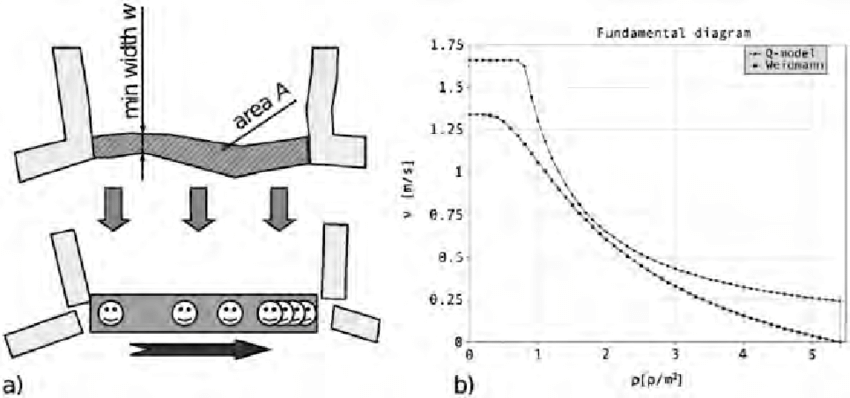
\includegraphics[width=\textwidth]{images/speed_lammel.png}
    \caption{rappresentazione modello di \textcite[]{lammel2010emergency}}
    \label{fig:asdkasdasd}
\end{figure}

Inoltre è stata considerata una velocità massima di 1.66 m/s poichè i valori considerati da Weidmann sono relativi
al flusso dei pedoni in condizioni normali e non in caso di emergenza.



\subsection{goto2012tsunami}
Una popolazione di 80,000 individui è stata considerata essi evacuano seguendo 
lo shortest path in base a nove delle possibili destinazioni di evacuazione alcune delle quali con una capacità limitata.

\vspace*{5mm}

Diversi scenari sono stati considerati in base al tempo di partenza o al numero di pedoni e auto
e la possibilità di cambiare la destinazione se il rifugio è pieno.

\vspace*{5mm}

Un agente intrappolato dallo tsunami presenta una velocità ridotta inversamente proporzionale in base
alla profondità dello tsunami viene stoppato e muore quando la profondità supera 1m.

\vspace*{5mm}

In questo lavoro diversi tipi di agenti sono modellati pedoni, motocicli e auto,
dove ogni agente rappresenta una famiglia.

\vspace*{5mm}

I pedoni sono suddivisi i pedoni normali con una velicità massima di 1.5 m/s,
mentre i pedoni lenti sono famiglie con handicappati, infanti o anziani con una velocità massima di 0.75 m/s.
le velocità sono ridotte all'aumentare della densità fino ad un massimo di 6 $p/m^2$.

\vspace*{5mm}

Per i motocicli una velocità massima di 30km/h è stata considerata con una densità massima di 0.9 $p/m^2$.

\vspace*{5mm}

Le auto in assenza di ostacoli si muovono per $L_{f} = V_{f} x \Delta_{t} $, dove $L_{f} = \textbf{free run length}$,
$V_{f} = \textbf{free run speed}$ e $\Delta_{t} = \textbf{time step}$
con un valore massimo di free run speed di 40 km/h è la velocità cambia in base
alla densità in fronte in particolare in base alla larghezza della strada.

\vspace*{5mm}

In caso di più corsie se una corsia è vuota in base alla density ahead l'auto allora può cambiare corsia,
per i pedoni e motocicli se la density ahead supera 1 $p/m^2$ occupano la corsia successiva sulla sinistra.

\vspace*{5mm}

In questo lavoro la densità in un'area davanti viene definita tramite la seguente formula
$\rho = n /(L \times W)$, dove $n$ è il numero di agenti nell'area $L \times W$, $L$ è la lunghezza di ricerca, 
che assume valori di 3m per i pedoni e 16.7m per i motocicli, e $W$ la larghezza della strada.
Per le auto la densità invece è definita nel seguente modo $\rho = n /((W - W_{c}) x L_{f})$, dove $W_{c}$ è la larghezza di un auto.

\vspace*{5mm}

Nel calcolo della densità un auto viene considerata 10 volte un pedone ed un motociclo 2 volte.
nel caso di interruzioni del traffico devono o aspettare o seguire il secondo shortest path.

\begin{figure}[ht]
    \centering
    \begin{subfigure}{0.45\textwidth}
        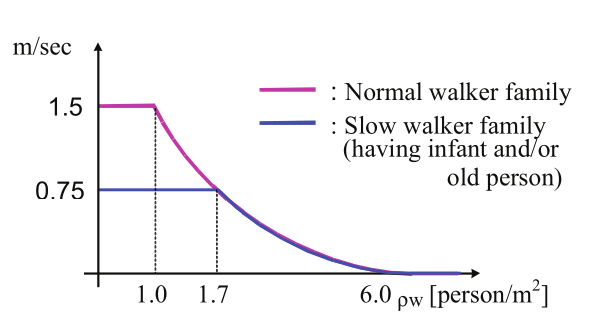
\includegraphics[width=\textwidth]{images/speed_GOTO.png}
        \caption{}
        \label{fig:adaads}
    \end{subfigure}
    \begin{subfigure}{0.45\textwidth}
        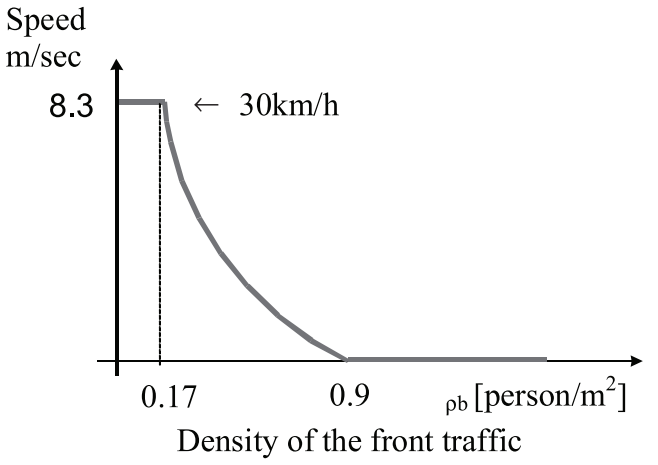
\includegraphics[width=\textwidth]{images/speed_GOTO_motocicli.png}
        \caption{}
        \label{fig:ssadada}
    \end{subfigure}
    \begin{subfigure}{0.45\textwidth}
        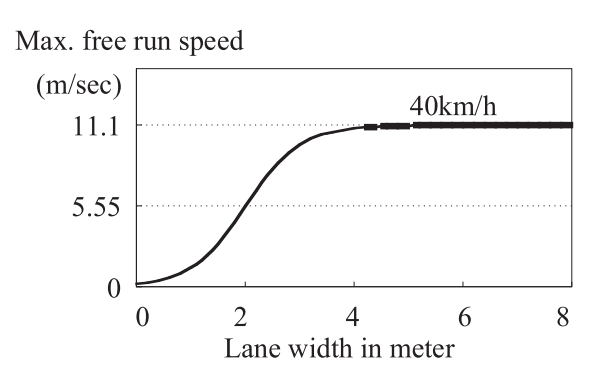
\includegraphics[width=\textwidth]{images/speed_GOTO_auto.png}
        \caption{}
        \label{fig:wrsnjds}
    \end{subfigure}
    \caption{Relazione velocità-densità: a) per i pedoni, b) motocicli e c) auto}
    \label{fig:ankdasndk}
\end{figure}



\subsection{takabatake2017simulated}
In questo lavoro un numero totale di 21,238 individui sono stati modellati, 
di cui due tipi di agenti sono stati distinti i residenti locali ed i visitatori.

\vspace*{5mm}

i residenti si assume che conoscano lo shortest path
per il rifugio più vicino dal punto in cui si trovano all'inizio dell'evacuazione.

\vspace*{5mm}

i visitatori invece seguono due regole seguendo un approccio probabilistico,
la prima regola “following other individuals” ad ogni intersezione seguono la strada con più individui,
la seconda regola “going to higher ground” ad ogni intersezione scelgono la strada che li porti ad un altezza maggiore.

\vspace*{5mm}

Sia i residenti che i pedoni vengono distinti in base all'età con una velocità massima di 1.19 m/s (Under 65) e 0.96 m/s (Over 65).
Basandosi sul lavoro di \textcite[]{older1968movement} hanno assunto una decrescità lineare della 
velocità da un livello di densità di 0.3 p/m² a uno di 3.0 p/m² (Fig. \ref{fig:speed-linear}).

\vspace*{5mm}

\begin{figure}[ht]
    \centering
    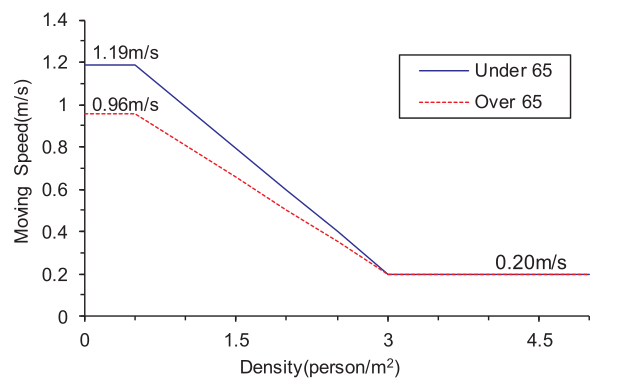
\includegraphics[width=0.7\textwidth]{images/speed_Linear.png}
    \caption{Relazione velocità-densità \textcite[]{takabatake2017simulated}}
    \label{fig:speed-linear2}
\end{figure}

\vspace*{5mm}

Due approcci sono stati utilizzati per decidere i tempi di partenza "all-togheter" dove tutti evacuano allo stesso tempo,
oppure una "delayed evacuation" in cui viene utilizzata la distribuzione di Rayleigh dove i parametri vengono decisi con dati provenienti da surveys.
Nessun cambiamento nei tempi di partenza viene gestito tra residenti e visitatori.

\vspace*{5mm}

I rifugi prevedono una capacità limitata, in caso fosse pieno al loro arrivo allora devono dirigersi allo shelter più vicino.
Gli autori hanno stimato che i visitatori abbiano un tempo di 30 secondi di attesa in cui chiedono informazioni sulla posizione dello shelter più vicino.

\vspace*{5mm}

Il casualty model utilizzato considera che un agente muore se l'altezza dell'inondazione alla sua posizione supera i 0.3 m.



\subsection{wang2021novel}

Questo lavoro considera tre diverse popolazioni al variare del numero di agenti 5000 e 10000,
che rappresentano la popolazione all'inizi dell'estate e 15000 rappresenta il picco estivo.

\vspace*{5mm}

Gli agenti distinti in pedoni e auto evacuano in base allo shelter più vicino a loro seguendo lo shortest path,
i rifugi in questo lavoro si assume abbiamo capacità illimitata.

\vspace*{5mm}

Il modello dei pedoni considera una velocità distribuita secondo una normale $\mathcal{N}(\mu_p,\sigma_p)$ troncata tra 0.75 m/s e 3.83 m/s e
con $\mu_p \sim \mathcal{U}(1.4, 2)$ e $\sigma_p \sim \mathcal{U}(0.1, 0.6)$, 
inoltre viene ridotta in base alla densità di fronte all'agente con una search length di 4m secondo l'andamento mostrato in figura \ref*{fig:dadknakdand}.

\begin{figure}[ht]
    \centering
    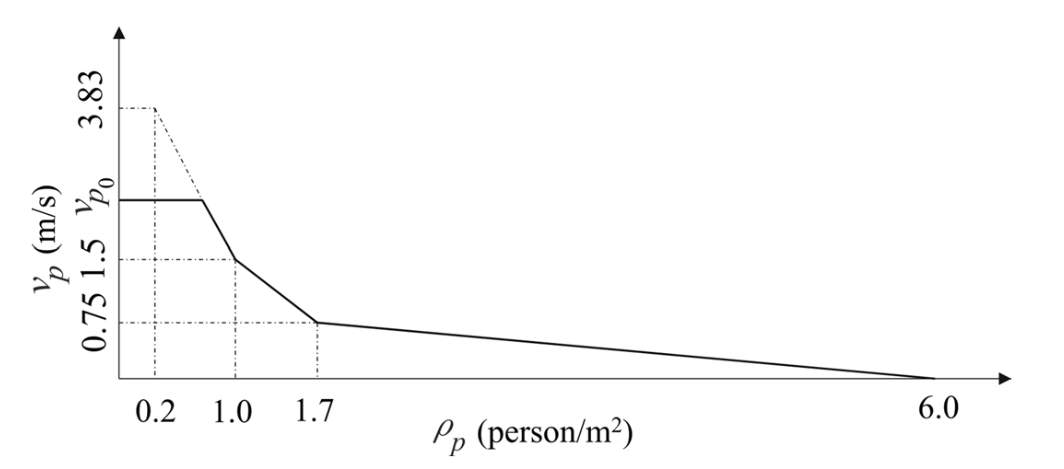
\includegraphics[width=0.7\textwidth]{images/speed_WANG.png}
    \caption{Relazione velocità-densità \textcite[]{wang2021novel} basato su un approssimazione del modello di \textcite[]{goto2012tsunami}}
    \label{fig:dadknakdand}
\end{figure}

Per le auto il modello di Greenshield è stato utilizzato in base alla densità di fronte lungo la free run length,
con una massima velocità di 40 km/h e densità massima di 160 veh/km per i link senza restrizioni sul traffico date dai danni sismici, altrimenti 120 veh/km.
Per il calcolo della densità si assume che ogni auto contenga 4 agenti ed che essa sia equivalente a 10 volte un pedone in spazio.

\vspace*{5mm}

Per la gestione delle interazioni tra auto e pedoni tre fasi di traffico vengono definite in base al rapporto
tra il volume dei pedoni e delle auto: \textit{vehicle-dominated}, \textit{balanced}, e \textit{pedestrian-dominated}.

\vspace*{5mm}

Per i tempi di partenza la distribuzione di Reylaight viene utilizzata dove $t_{0}$ segue una distribuzione uniforme in [3, 10] (unit: min)
$\tau$ and $\sigma_{t}$ seguono una distribuzione uniforme in [0, 10] (unit: min) e [1, 5] rispettivamente, 
inoltre per maggior realismo gli agenti devono recarsi prima a degli appositi parcheggi per poter evacuare in auto.

\vspace*{5mm}

Rispetto ai lavori passati che utilizzvano un livello di profondità fissa $h_c$ per determinare la morte degli agenti,
viene considerato che $h_c$ segua una distribuzione uniforme in [0.5, 3] (unit: m). 

\vspace*{5mm}

descrizione modello terremoto


\newpage
